\section{Regression Analysis in Practice}
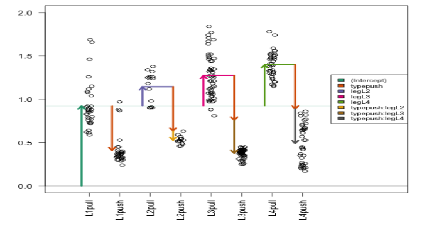
\includegraphics[width=\columnwidth]{did}

\subsection*{Categorical Variables}
\textbf{Treatment and Control Group: } \\
$Y_i=\alpha+\beta D_i + \gamma X_i + \epsilon_i$\\
In this case $\beta$ is the difference in intercept between group \textbf{\textit{A}} and group \textbf{\textit{B}}. This is the most frequent way that RCT are analyzed: the matrix X are "control" variables. 

\subsection*{Difference-in-Difference}
\textbf{\{Treatment, Control\}$\times$\{Male, Female\}: } \\
$Y_i=\alpha+\beta D_i + \gamma M_i + \delta M_i \ast D_i + \epsilon_i$ \\
So, $\delta$ is the difference between group \textbf{\textit{Male}} and group \textbf{\textit{Female}} in difference between group \textbf{\textit{Treatment}} and group \textbf{\textit{Control}}. \\
\textit{\textbf{Assumption: }Parallel trends assumption. }\\
\textit{\textbf{Causal interpretation: }If you cannot credibly claim that the parallel trends assumption is satisfied, then estimates obtained from a differences-in-differences design cannot be interpreted causally. }

\subsection*{Local Linear Regression}
\begin{itemize}
    \item Define the dummies as: \\
    $D_{1i} = I_{X_0 \leq X_{1i} < X_1}$\\
    $D_{2i} = I_{X_1 \leq X_{1i} < X_2}$
    \item Run regression: \\
    $Y_i=\beta_1 D_{1i} + \beta_2 D_{2i} + \dots + \beta_J D_{Ji} + \epsilon_i$
    \item Define Piece wise linear variables. 
\end{itemize}

\subsection*{Omitted Variable Bias}
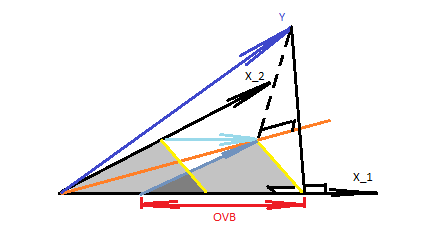
\includegraphics[width=\columnwidth]{ovb}
Correct model: $Y_i=\beta_0+\beta_1 X_{1i}+\beta_2 X_{2i}+\epsilon_i$\\
Estimated model: $Y_i=\alpha_0+\alpha_1 X_{1i}+w_i$\\
Define Ancillary (or Auxillary) regression: $X_{2i}=\delta_0+\delta_1 X_{1i}+\zeta_i$\\
Then,\\
${OVB}=\hat{\alpha_1}-\beta_1=\delta_1 \beta_2$
